% The historical Henry Cavendish's experiment (1798) to determine the gravitational constant G
% and hence the mean density of the Earth.
%
\documentclass[tikz, border = 1 cm]{standalone}
\usepackage{tikz}

\usepackage{tkz-euclide}

\begin{document}
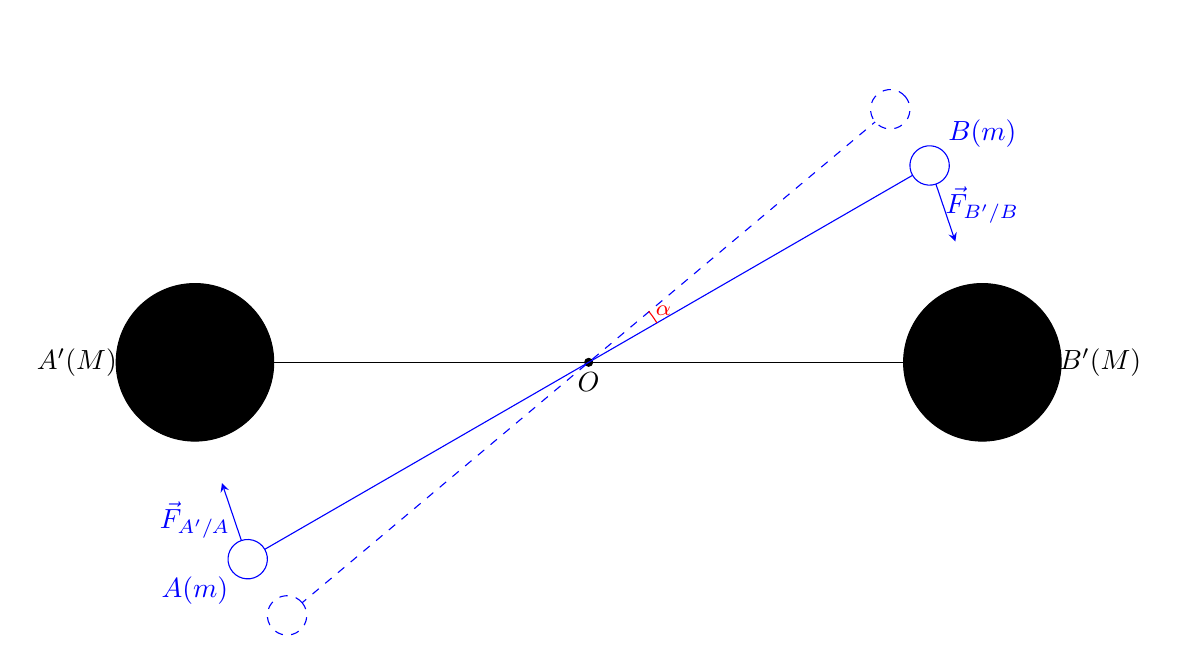
\begin{tikzpicture}
  %Torsion balance with arrows for forces
      \newcommand{\torsion}[1][2]
                 {\draw[#1,color=blue] (-5,0)--(5,0);
                   \draw[#1,color=blue,>=stealth,->] (-5,0) -- (-4.8,1);
                   \draw[#1,color=blue,>=stealth,->] (5,0) -- (4.8,-1);
                  \filldraw[#1,color=blue, fill=white] (-5,0) circle (0.25);
                  \filldraw[#1,color=blue, fill=white] (5,0) circle (0.25);
                 }

  %Torsion balance dashed
      \newcommand{\torsionDashed}[1][2]
                 {\draw[#1,dashed, color=blue] (-5,0)--(5,0);
                  \filldraw[#1,dashed, color=blue, fill=white] (-5,0) circle (0.25);
                  \filldraw[#1,dashed, color=blue, fill=white] (5,0) circle (0.25);
                 }
                 
      \tkzDefPoint(0,0){E}
      \tkzDefPoint(-5,0){A1}
      \tkzDefPoint(5,0){A2}
      \tkzDrawSegments(A1,A2)
      \filldraw (E) circle (0.05);
      \torsion[shift={(0,0)}, rotate=30];
      \torsionDashed[shift={(0,0)}, rotate=40];

      %Lead balls
      \filldraw (A1) circle (1);
      \filldraw (A2) circle (1);

      %The angle alpha
      \begin{scope}
        \clip (E)  -- (5,2.9) -- (5,4.25) -- cycle;
        \draw [red] (E) circle (1);
        \node[red] at (0.95,0.65) {\footnotesize $\alpha$};
      \end{scope}

      %Labels
      \node[below] at (E) {$O$};
      \node[blue] at (5,2.9) {$B(m)$};
      \node[blue] at (-5,-2.9) {$A(m)$};
      \node[blue] at (-5,-2) {$\vec{F}_{A'/A}$};
      \node[blue] at (5,2) {$\vec{F}_{B'/B}$};
      \node at (-6.5,0) {$A'(M)$};
      \node at (6.5,0) {$B'(M)$};
\end{tikzpicture}
\end{document}
